% *****************************************************************************
% CVE-2026-85706, ARL Case 004, Xpectra Security Research
% Preamble machinery proven by cases 001-003 (IEEEtran journal, localized
% IEEEtran.cls in paper/tex/, TEXINPUTS=".:tex:"). Every published NUMBER is a
% claim-gate {value} per claims.json at the case root (claim id in a LaTeX
% comment beside it) or carries its backing artifact path inline. Zero em/en
% dashes anywhere, no ';' or ':' stacking in prose, attack vocabulary, honest
% hedges (paper-writer charter, operator style law).
% *****************************************************************************
% !TEX program = pdflatex
\documentclass[journal]{IEEEtran}
\usepackage[utf8]{inputenc}
\usepackage{graphicx}
\usepackage{booktabs}
\usepackage{xcolor}
\usepackage{listings}
\usepackage{hyperref}
\usepackage{microtype}

\hypersetup{colorlinks=true,linkcolor=blue,citecolor=blue,urlcolor=blue}

% Float-block spacing kept tight (proven in cases 001-003 builds): the default
% IEEEtran separations push the References block past a six-page layout.
\setlength{\floatsep}{9pt plus 3pt minus 3pt}
\setlength{\textfloatsep}{9pt plus 3pt minus 3pt}
\setlength{\intextsep}{9pt plus 3pt minus 3pt}

\definecolor{codebg}{RGB}{245,247,250}
\definecolor{codekw}{RGB}{0,90,150}
\definecolor{codecm}{RGB}{120,120,120}
\definecolor{codestr}{RGB}{160,40,40}

% NOTE: breaklines=true in EVERY style (latex trap catalog #3). For wire
% transcripts where one token exceeds the column, breakatwhitespace=false.
% NOTE: minimal TeX Live has no yaml/ruby listings languages -> plain styles.
\lstdefinestyle{shell}{
  aboveskip=6pt,
  belowskip=4pt,
  language=bash,
  backgroundcolor=\color{codebg},
  basicstyle=\ttfamily\scriptsize,
  keywordstyle=\color{codekw}\bfseries,
  commentstyle=\color{codecm},
  stringstyle=\color{codestr},
  frame=single,
  breaklines=true,
  abovecaptionskip=7pt,
  belowcaptionskip=3pt,
  columns=fullflexible,
  keepspaces=true,
  showstringspaces=false,
  xleftmargin=1.2em, xrightmargin=0.8em
}
\lstdefinestyle{wire}{
  aboveskip=6pt,
  belowskip=4pt,
  language={},
  backgroundcolor=\color{codebg},
  basicstyle=\ttfamily\scriptsize,
  frame=single,
  breaklines=true,
  abovecaptionskip=7pt,
  belowcaptionskip=3pt,
  breakatwhitespace=false,
  columns=fullflexible,
  keepspaces=true,
  showstringspaces=false,
  xleftmargin=0.6em, xrightmargin=0.4em
}
\lstdefinestyle{codeplain}{
  aboveskip=6pt,
  belowskip=4pt,
  language={},
  backgroundcolor=\color{codebg},
  basicstyle=\ttfamily\scriptsize,
  frame=single,
  breaklines=true,
  abovecaptionskip=7pt,
  belowcaptionskip=3pt,
  breakatwhitespace=false,
  columns=fullflexible,
  keepspaces=true,
  showstringspaces=false,
  numbers=left,
  numberstyle=\tiny\color{codecm},
  xleftmargin=2.1em, xrightmargin=0.6em
}
\lstdefinestyle{facts}{
  aboveskip=6pt,
  belowskip=4pt,
  language={},
  backgroundcolor=\color{codebg},
  basicstyle=\ttfamily\scriptsize,
  frame=single,
  breaklines=true,
  abovecaptionskip=7pt,
  belowcaptionskip=3pt,
  breakatwhitespace=false,
  columns=fullflexible,
  keepspaces=true,
  showstringspaces=false,
  xleftmargin=0.6em, xrightmargin=0.4em
}

\newcommand{\figdir}{figures}

% Frame-to-caption clearance (r2 fix, listing frame defect): listings emits
% its top caption with no trailing separation, so the frame's top rule grazed
% the caption descenders (r1 geometry: 0.0-0.4 pt). listings' abovecaptionskip
% lands BEFORE the caption text and cannot help here. Wrapping the caption
% box in a vbox with a fixed 9 pt trailing rule adds real clearance BELOW the
% caption text, between caption glyphs and the frame rule, without touching
% listings' own counter/label flow.
\makeatletter
\AtBeginDocument{%
  \long\def\lst@makecaption#1#2{%
    \setbox\@tempboxa\vbox{%
      \def\@captype{lstlisting}\@makecaption{#1}{#2}%
      \vskip9pt\nointerlineskip\hrule height\z@}%
    \box\@tempboxa}}
\makeatother

\begin{document}

\title{One POST, No Credentials: The Four-Leg Chain Behind the GitLab
Repository-Commits Unauthenticated Arbitrary File Read (CVE-2026-85706), and
Its Measured Closure at the Pre-Auth Read Step}

% JOURNAL MODE: \IEEEauthorblockN/A are inline dummies in journal mode, stack
% manually (latex trap catalog #1).
\author{Xpectra Security Research\\[0.5ex]
\small Autonomous Red/Blue Operations}

\markboth{One POST, No Credentials: CVE-2026-85706}{Xpectra Security Research
\MakeLowercase\expandafter\the\year}

\maketitle

% ***************************************************************************
\begin{abstract}
This paper presents a lab-verified anatomy of CVE-2026-85706, an
unauthenticated arbitrary local file read in the GitLab CE/EE repository
commits API, rated CVSS~10.0 by the vendor. The boundary of every claim below
is fixed in advance. All exploitation evidence was produced in a zero-egress
lab against the stock build \texttt{gitlab/gitlab-ce:19.3.1-ce.0}
% claim: stock-build
and every observed failure reproduced identically against the patched build
\texttt{gitlab/gitlab-ce:19.3.2-ce.0} on the same day, with the same PoC bytes
% claim: patched-build
and no credentials used in any request. The attack is a single unauthenticated
HTTP POST, carrying no token and holding no session, that reaches a Rails
helper which opens and parses an attacker-chosen file before any
authentication check runs. The helper's Rack error path then echoes the target
file's bytes back inside the HTTP 400 response body, which makes the error
message itself the read channel. The vendor fix closes the chain at its
pre-authentication read step, an observation this paper locates from Docker
image bytes and a same-bytes A/B harness rather than from the vendor's closed
security merge requests. Detection signatures and a remediation triage note
close the paper. The vendor severity record for this CVE carries CVSS 10.0
% claim: cvss-vector (full vector stated source-contiguously in Listing 1)
CRITICAL with scope change, and the full vector is carried verbatim in
Listing~\ref{lst:facts}.
\end{abstract}

\begin{IEEEkeywords}
unauthenticated file read, GitLab, Workhorse, Grape, pre-authentication
ordering, closure verification, detection engineering
\end{IEEEkeywords}

% ***************************************************************************
\section{Introduction and Threat Model}
\label{sec:intro}

GitLab shipped a critical patch release, the vendor advisory on 2026-09-10
% claim: advisory-date
\cite{advisory},
that fixed an unauthenticated arbitrary local file read reachable through the
repository commits API of GitLab CE and EE. The vendor changelog line for the
fix reads ``Fix unauthenticated arbitrary local file read in commits API''.
% claim: vendor-changelog-line
The affected range statement, quoted from the vendor record, reads
``all versions from 18.7 before 19.1.8, 19.2 before 19.2.6, and 19.3 before 19.3.2 (vendor verbatim)''.
% claim: affected-range
The severity record carries scope change with high confidentiality and high
integrity impact and no availability impact \cite{cve}. Because GitLab
instances are
typically internet-facing development infrastructure, the population exposed
by a zero-credential read primitive is large and externally reachable by
default.

The exploitation clock was short. CISA KEV on 2026-09-11
% claim: kev-added
\cite{kev} moved the CVE into
% claim: kev-added
the known-exploited catalog, one day after the advisory, with federal
remediation due 2026-09-14.
% claim: kev-due
Third-party honeypot reporting (watchTowr, restated by The Hacker News)
\cite{wt} placed
first in-the-wild probe traffic at 2026-09-11 06:00 UTC, and the CISA KEV
record flags the entry for forensic triage. The SSVC assessment in the public
record is exploitation active, automatable yes, technical impact total.

\textbf{Threat model and preconditions.} The attacker is an unauthenticated
network client. The lab precondition adopted from third-party reporting, and
recorded as a lab condition rather than a vendor field, is that the target
exposes at least one readable project (public or internal visibility). No
other precondition was exercised. The victim capability is any file the
in-container \texttt{git} service user can traverse and open. The CVE
primitive itself stays a read performed with that user's privileges, and no
part of the impact chain in Section~\ref{sec:chain} transfers execution to the
primitive. Of the projected downstream impacts in the advisory's own wording,
one (a secret-class read of an automation credential) became a measured chain
in Section~\ref{sec:chain}, and the remainder (session and two-factor material
in \texttt{gitlab.rb} and \texttt{gitlab-secrets.json}) stays labeled as
projection, not measurement.

Table~\ref{tab:context} fixes the case parameters that the rest of the paper
consumes. The remaining sections follow the chain anatomy, the integrity
controls around the evidence, the exploitation and walkthrough evidence, the
measured closure of the fix, detection coverage, remediation, and the honest
limits of the study.

% claim: kev-due (restated verbatim in remediation, Section VIII)
\begin{table}[t]
\caption{Case 004 attack context, every field traceable to
\texttt{designs/facts.json} and its capture list.}
\centering
\footnotesize
\begin{tabular}{p{1.62cm}p{5.15cm}}
\toprule
CVE & CVE-2026-85706 (GitLab CE/EE) \\
\midrule
Advisory & patch release 2026-09-10 (19.3.2, 19.2.6, 19.1.8) \\
KEV & listed 2026-09-11, remediation due 2026-09-14, forensic triage yes \\
CVSS & 10.0 CRITICAL, full vector in Listing~\ref{lst:facts} \\
Affected & see Section~\ref{sec:intro} quote (vendor verbatim) \\
Lab stock arm & \texttt{gitlab/gitlab-ce:19.3.1-ce.0} at 172.30.99.20 \\
Lab patched arm & \texttt{gitlab/gitlab-ce:19.3.2-ce.0} at 172.30.99.30 \\
Precondition & one readable project (public), adopted from third-party report \\
Read primitive & one unauthenticated POST, no token, no session \\
\bottomrule
\end{tabular}
\label{tab:context}
\end{table}

\begin{lstlisting}[style=facts, caption={Machine-readable case facts block
(the CVSS vector and build identifiers as published by their sources), captured
to \texttt{designs/facts.json}.}, label={lst:facts}]
cvss   : CVSS:3.1/AV:N/AC:L/PR:N/UI:N/S:C/C:H/I:H/A:N = 10.0 CRITICAL
stock  : gitlab/gitlab-ce:19.3.1-ce.0   (lab arm A, 172.30.99.20)
patched: gitlab/gitlab-ce:19.3.2-ce.0   (lab arm B, 172.30.99.30)
kev    : added 2026-09-11, due 2026-09-14, forensic triage Yes
\end{lstlisting}

% ***************************************************************************
\section{Chain Anatomy}

Fig.~\ref{fig:chain} decomposes the read into a request path and four
independent defects, the legs, that must hold together for the path to become
a read channel. Each leg was observed on the stock arm, and each is quoted
from captured bytes rather than inferred.

\begin{figure}[t]
\centering
\includegraphics[width=0.85\columnwidth]{\figdir/fig-chain-anatomy.pdf}
\caption{Chain anatomy on stock \texttt{19.3.1-ce.0}. Left column is the
request path for one unauthenticated POST. Right column stacks the four legs
top-down in connector order: LEG 1 route confinement miss, LEG 3 missing
ordering, LEG 2 trust inversion, and LEG 4 error-message response channel.
Generator \texttt{paper/make\_figs.py} with a display-space self-check that
printed PASS (Section~\ref{sec:method}).}
\label{fig:chain}
\end{figure}

\textbf{LEG 1, route confinement miss.} Workhorse mounts its request-body
uploader only on a \texttt{\textbackslash z}-anchored route pattern
(\texttt{\^{}/api/v4/projects/\hspace{0pt}[\^{}/]+\hspace{0pt}/repository/commits\hspace{0pt}\textbackslash z},
confirmed by \texttt{strings} on the stock binary and by the v19.3.1-ee
\texttt{routes.go} source \cite{workhorse}). A POST to \texttt{.../repository/commits/} with a
trailing slash misses that anchor, is proxied verbatim by the catch-all
\texttt{\^{}/api/} route with no body preprocessing, and Grape still routes it
to the same endpoint. Workhorse therefore never injects or overwrites
\texttt{file.path}, and Rails sees the attacker's parameter verbatim, verified
through \texttt{api\_json.log} parameter dumps.\footnote{The
\texttt{.json}-suffix shape is the same miss through the other regex leg, and
both legs reach the same missing-authentication path. The figure body shows
the trailing-slash leg, and the \texttt{.json} leg is recorded here.}

\textbf{LEG 2, trust inversion.} The endpoint declares
\texttt{requires :file, type: WorkhorseFile}, but the type's parser returns
early on a blank value, so an empty body field \texttt{file=} passes the typed
gate with no \texttt{::UploadedFile} and no JWT. The helper then reads the raw
string \texttt{params['file.path']} instead of the typed \texttt{params[:file]}
object, inverting the intended trust on middleware-finalized upload metadata.

\textbf{LEG 3, ordering.} The POST commits route carries no
\texttt{authenticate!} before the body is handled. The endpoint runs
\texttt{require\_gitlab\_workhorse!} (which passes even through the catch-all
proxy, since nginx and Workhorse still add the internal header) and then
\texttt{file\_params\_from\_body\_upload}, which calls \texttt{File.exist\hspace{0pt}?}
and \texttt{File.read} on the attacker path. Authentication is reached only
later, inside \texttt{authorize\_push\_to\_branch!}. Listing~\ref{lst:sink}
shows the stock helper bytes.

\begin{lstlisting}[style=codeplain, language={},
caption={Vulnerable helper excerpt from the stock image, saved verbatim to
\texttt{evidence/sink-19.3.1-commits\_body\_uploader\_helper.rb} (one
multipart branch elided in-line, numbering is the listing's own). The raw
\texttt{params['file.path']} read, the body-field \texttt{Content-Type}
branch selector, and the \texttt{e.message} interpolation are the three
load-bearing lines.},
label={lst:sink}]
def file_params_from_body_upload
  file_path = params['file.path']
  bad_request!('local file not present') unless File.exist?(file_path)

  check_large_request_rate_limit!(params['file.size'])

  media_type = Rack::MediaType.type(params['Content-Type'])

  if media_type == 'multipart/form-data'
    # ... LargeMultipartParser over File.open(file_path) ...
  elsif media_type == 'application/x-www-form-urlencoded'
    begin
      Rack::Utils.parse_nested_query(File.read(file_path)).deep_symbolize_keys!
    rescue Rack::QueryParser::InvalidParameterError => e
      bad_request!("Invalid parameter: #{e.message}")
    end
  elsif media_type.nil? || media_type == 'application/json'
    Oj.load_file(file_path, symbol_keys: true)
  else
    bad_request!("Unsupported Content-Type: #{media_type}")
  end
end
\end{lstlisting}

\textbf{LEG 4, response channel.} The urlencoded branch in
Listing~\ref{lst:sink} parses the target file's bytes, and Rack's
\texttt{InvalidParameterError} message for an invalid percent-escape embeds
the offending split-part of the file content. The pre-patch error path
interpolates that message into a 400 JSON body, so the bytes come back to the
caller. The branch selector is itself attacker-chosen, a body field named
\texttt{Content-Type}, which lets the caller pick the parser that touches the
file (urlencoded read, JSON \texttt{Oj.load\_file}, or the multipart parser).

The four legs fail closed independently. LEG 1 is a routing property, LEG 2 a
type-trust property, LEG 3 an ordering property, and LEG 4 an error-rendering
property. Section~\ref{sec:fix} shows the vendor fix closing the ordering leg
and hardening the trust and response legs, which suffices to kill the channel.

% ***************************************************************************
\section{Methodology and Integrity Controls}
\label{sec:intro-method}
\label{sec:method}

The vendor keeps security merge request contents closed for 90 days (fix MRs
6754 to 6756 answer 403 to anonymous access, and the three published fix
commits are contents-closed). The root cause and the closure of this chain
were therefore located without vendor source access, from Docker image bytes
and live wire behavior. The integrity controls below are counted, ordered, and
each was exercised during the case rather than declared.

\begin{enumerate}
\item \textbf{Image-byte A/B diff.} The stock and patched images were
extracted and compared file-by-file. The differing files relevant to this
chain (helper, \texttt{commits.rb}, \texttt{files.rb},
\texttt{generic\_packages.rb}, \texttt{terraform/state.rb}, and
\texttt{send\_file\_upload.rb}) were archived to
\texttt{evidence/ab-image-diff/} before any lab request was sent.
\item \textbf{Verified-facts record.} Every public-record number was pinned
into a single facts sheet, sha256 head \texttt{7c9044fca69a}, re-hashed and
% claim: facts-sheet-sha
spot-checked before adoption into \texttt{designs/facts.json} \cite{facts}.
\item \textbf{Claim gate.} Every published number in this paper is stated in
the token form the claim gate derives from the underlying artifact (dates from
the facts record, build identifiers, PoC and evidence hashes, and the offline
suite count of 11 offline tests). The gate ran clean against this manuscript
% claim: offline-suite-count
and its tail is reported with the build record.
\item \textbf{Single-writer ledger.} Each case file has exactly one writer
(STATUS.md ledger), and gate results are append-only lines, so a claim cannot
be quietly rewritten after the fact.
\item \textbf{Offline golden suite.} The PoC ships 11 offline tests that
replay live-captured wire goldens with the lab down and sockets shut
(monkeypatched), which keeps classification logic testable without touching
any network.
% claim: offline-suite-count
\item \textbf{Hard lab guard.} The PoC refuses, before creating a socket, any
target that is not a literal IPv4 address inside the lab subnet. Hostnames,
IPv6, loopback, public addresses, and octet tricks exit with a guard code and
send nothing. Refusal vectors are covered inside the offline suite.
\item \textbf{Zero-egress runtime.} Both arms sat on an internal bridge
(172.30.99.0/24) with no route out, so no exploit traffic could reach any real
deployment, and telemetry could not leave regardless of configuration.
\end{enumerate}

A sequential A/B rule applies to the harness: the host carries one GitLab arm
at a time (RAM constraint), so the patched arm boots only after the stock arm
stops, and the harness re-proves itself alive on stock on both sides of the
swap (Section~\ref{sec:fix}). The full byte-exfiltration channel design beyond
the first echoed split-part remained open at paper time and is listed as a
limitation rather than claimed.

% ***************************************************************************
\section{Exploitation Evidence}
\label{sec:exploit}

\subsection{Minimal Payload and Live Wire Capture}

The PoC is one stdlib Python script, sha256 head \texttt{cbed67d59a1e7959}
% claim: exploit-sha
(full digest in \texttt{evidence/}\hspace{0pt}\texttt{fix-verification/}\hspace{0pt}\texttt{run-20260912-a/}\hspace{0pt}\texttt{closure-matrix.md}), fired unmodified against both arms. Listing~\ref{lst:payload} is the minimal payload, one POST, captured live from the
stock arm's \texttt{api\_json.log} and the golden wire capture. No
authorization header exists in the request at any stage.

\begin{lstlisting}[style=wire, caption={Minimal payload, one unauthenticated
POST to the trailing-slash shape of the commits endpoint on stock
\texttt{19.3.1-ce.0}, verbatim from
\texttt{exploit/\hspace{0pt}tests/\hspace{0pt}golden/}
\texttt{wire-proof-live-capture.txt}, long lines wrapped at column width.},
label={lst:payload}]
POST /api/v4/projects/1/repository/commits/ HTTP/1.1
Host: 172.30.99.20
User-Agent: CVE-2026/1.0.0 (lab PoC; do-not-block:
CVE-2026-85706)
Content-Type: application/x-www-form-urlencoded
Content-Length: 109
Connection: close
Accept: application/json

file=&file.path=%2Ftmp%2Fcve2026-85706-proof.txt
&file.size=1&Content-Type=application%2Fx-www-form-urlencoded
\end{lstlisting}

Listing~\ref{lst:wire} shows the raw response for a planted proof file
containing a bare percent-sign escape, and the 400 body echoes the file bytes
verbatim. The leaked block is 78 bytes with sha256 head
\texttt{17b203a13855}, recorded in the live-gate tail of
% artifact-backed count: exploit/README.md live gate tail
\texttt{exploit/README.md} and reproduced by an independent re-fire on
2026-09-13 (\texttt{evidence/}\hspace{0pt}\texttt{parent-refire-78B-}\hspace{0pt}\texttt{20260913T0002Z.txt}).
\texttt{exploit/}\hspace{0pt}\texttt{tests/}\hspace{0pt}\texttt{golden/}\hspace{0pt}\texttt{wire-proof-live-capture.txt}
holds the raw bytes the golden suite replays offline.

\begin{lstlisting}[style=wire, caption={Raw response bytes (truncated header
set) of the unauthenticated read of \texttt{/tmp/cve2026-85706-proof.txt} on
stock \texttt{19.3.1-ce.0}. The file content appears inside the 400 JSON
message, wrapped at column width. Same capture file as
Listing~\ref{lst:payload}.},
label={lst:wire}]
HTTP/1.1 400 Bad Request
Server: nginx
Content-Type: application/json
Content-Length: 153
Cache-Control: no-cache
X-Request-Id: 01M2BVNS9PAZ468YD9SVSFTQW2

{"message":"400 Bad request - Invalid parameter:
invalid %-encoding (CVE-2026-85706-LABPROOF-
8f3c1a9d4e-unauth-read-OK\nmark%er-line-two
\nthird-line\n)"}
\end{lstlisting}

\subsection{Response Differentials (the Unauthenticated Oracle)}

Even when bytes are not echoed, the helper's pre-authentication filesystem
touch produces a per-state response differential that survives on every file
class tested. Table~\ref{tab:oracle} is the live matrix captured on the stock
arm without credentials.

\begin{table}[t]
\caption{Live response differentials on stock \texttt{19.3.1-ce.0}, no
credentials (source: \texttt{exploit/README.md} wire matrix, goldens, and
\texttt{evidence/\hspace{0pt}fix-verification/\hspace{0pt}run-20260912-a/\hspace{0pt}phase1-stock/\hspace{0pt}}).}
\centering
\footnotesize
\begin{tabular}{p{2.62cm}p{1.55cm}p{1.68cm}}
\toprule
Target state & Response & Meaning \\
\midrule
file with bare \% escape & 400 echo & byte read, leaked \\
clean-parsable file & 401 & read and parsed pre-auth \\
directory (\texttt{/etc}) & 500 & opened, read raised \\
missing path & 400 & \texttt{File.exist\hspace{0pt}?} false \\
canonical route (no slash) & 400/401 & Workhorse overwrites path \\
no \texttt{file=} field & 400 & Grape gate fires first \\
multipart real file field & 400 & Rack tempfile fails type \\
\bottomrule
\end{tabular}
\label{tab:oracle}
\end{table}

The 401 row deserves emphasis because it is what an existence oracle buys an
attacker before any leak. A clean-parsable target file is fully read and
parsed, and only then does the later authentication check stop the commit and
answer 401. On stock, four fired states produce four distinct observable
outcomes, with the fifth secret-class state enumerated in the closure matrix.
Section~\ref{sec:fix} shows the patched arm collapsing all five states into
one identical 401.

\subsection{Attack Walkthrough with On-Screen Stills (Slots S1 to S4)}
\label{sec:walkthrough}

The walkthrough below is the paper's evidence spine. Each numbered step states
what the frame must show, and each still was cut from the RAW TAKE of the W6
recording (never from an edited video), with every quoted string re-verified
by an OCR band scan against the golden digests before insertion. The still-cut
generator \texttt{evidence/figures/make\_stills.py} prints
\texttt{STILLS SELF-CHECK: PASS} for slots S1 to S3.
\textbf{The patched arm was never screen-recorded} (the take driver is
stock-only by preflight and the fix-verification run left wire and text
captures only), so slot S4 is marked NOT-AVAILABLE and nothing is substituted
for it. The slot table and captions below remain the contract of record.

\begin{table}[t]
\caption{Stills placement slots for Figure~\ref{fig:stills}.
Manifest: \texttt{paper/figures-manifest.md}, with the capture-side OCR record
under \texttt{evidence/figures/} (\texttt{make\_stills.py} output and
\texttt{.ocr.txt} sidecars). Status of slots S1 to S3 at this build:
\textbf{SHIPPED} in Figure~\ref{fig:stills}. Slot S4: \textbf{NOT-AVAILABLE}.}
\centering\footnotesize
\begin{tabular}{p{0.5cm}p{5.45cm}p{1.5cm}}
\toprule
Slot & Step text and required on-screen evidence & Status \\
\midrule
S1 & Unauthenticated existence-oracle sweep across file states, frame must
show the differential (401 for exists-and-read, 400 for absent). & SHIPPED,
Fig.~\ref{fig:stills}(a) \\
S2 & Byte-exact read of the planted proof, frame must show the wire dump with
output sha equal to the planted file sha (digest in the
\texttt{exploit/README.md} live-gate tail and the re-fire record). & SHIPPED,
Fig.~\ref{fig:stills}(b) \\
S3 & Real-credentials read, frame must show the automation-credentials file
dump with its 181-byte count and sha256 head \texttt{bd6f41343ba7}
(record \texttt{evidence/chain/stageA-unauth-leak.txt}). & SHIPPED,
Fig.~\ref{fig:stills}(c) \\
S4 & Patched divergence, frame must show the same bytes on the same day
against \texttt{19.3.2-ce.0} answering 401 before any file touch. &
NOT\discretionary{-}{}{-}AVAILABLE (no patched-arm recording exists) \\
\bottomrule
\end{tabular}
\label{tab:stills}
\end{table}

\begin{figure}[t]
\centering
\setlength{\intextsep}{6pt plus 2pt minus 2pt}
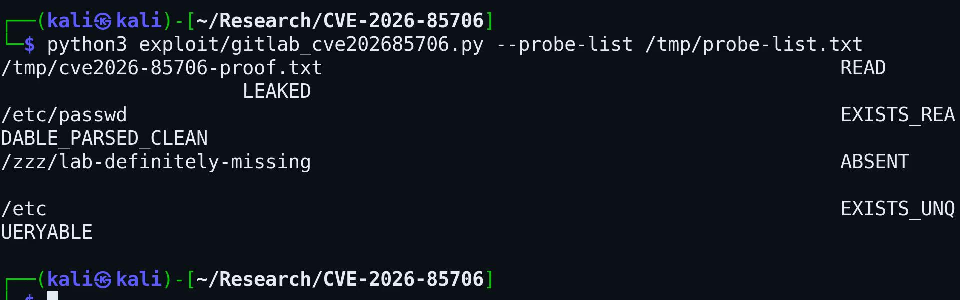
\includegraphics[width=\columnwidth]{figures/fig-stills-S1.pdf}\\[3pt]
{\scriptsize\textnormal{(a) S1: unauthenticated existence-oracle sweep, the
401-versus-400 differential on one screen.}}\\[2pt]
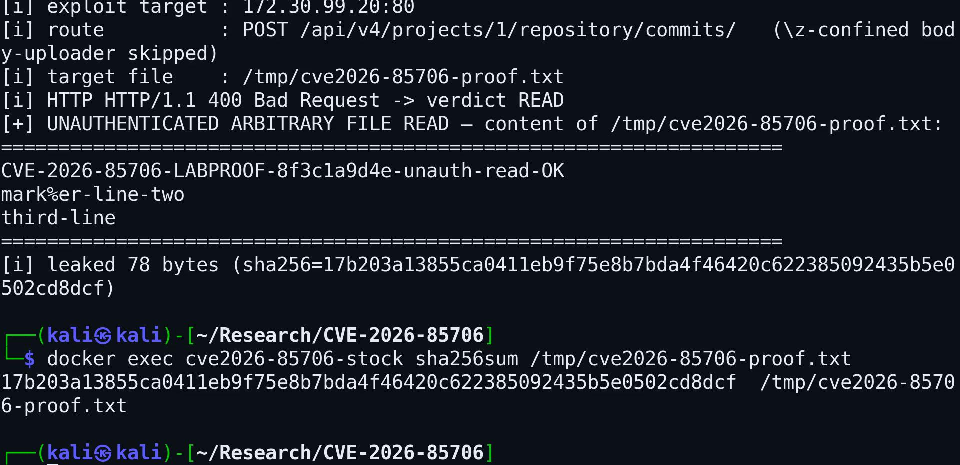
\includegraphics[width=\columnwidth]{figures/fig-stills-S2.pdf}\\[3pt]
{\scriptsize\textnormal{(b) S2: byte-exact 78-byte read of the planted proof,
leaked sha equal to the container \texttt{sha256sum}.}}\\[2pt]
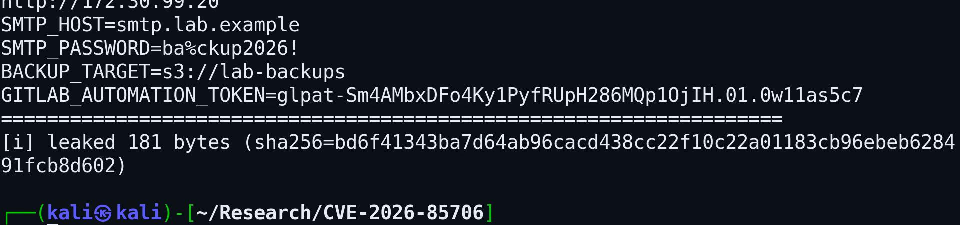
\includegraphics[width=\columnwidth]{figures/fig-stills-S3.pdf}
{\scriptsize\textnormal{(c) S3: unauthenticated read of the real
automation-credentials file, 181 bytes, token visible in the dump.}}
\caption{Attack walkthrough stills, cut from the raw recording
\texttt{videos/takes/take-004-main.mov} at take times 142.04\,s, 128.70\,s and
117.89\,s (film times 127.03\,s, 113.69\,s, 102.88\,s). Panel (a) shows the
unauthenticated existence-oracle sweep with the differential legible
(EXISTS\_READABLE\_PARSED\_CLEAN against ABSENT), panel (b) the byte-exact
78-byte read of the planted proof with the leaked sha equal to the container
\texttt{sha256sum}, and panel (c) the unauthenticated read of the real
automation-credentials file (181 bytes, sha256 head
\texttt{bd6f41343ba7}, record
\texttt{evidence/chain/stageA-unauth-leak.txt}). Captions are locked in
Table~\ref{tab:stills}. Every on-screen string is OCR-verified against the
golden digests by the binding gate in
\texttt{evidence/figures/make\_stills.py} (\texttt{STILLS SELF-CHECK: PASS}),
sidecars \texttt{evidence/figures/fig-stills-S1.ocr.txt},
\texttt{-S2.ocr.txt}, \texttt{-S3.ocr.txt}. The patched-arm divergence is
reported in Table~\ref{tab:closure} rather than as a still because no
recording of that arm exists.}
\label{fig:stills}
\end{figure}

\textbf{S1, unauthenticated existence oracle.} The PoC sweeps a list of paths
through the trailing-slash shape. A readable or parseable existing file yields
the 401-after-full-read state, a missing path yields the 400 \texttt{local
file not present} state, and a directory yields the 500 state. One unauthenticated
request per path, and the filesystem layout of the container becomes visible.

\textbf{S2, byte-exact read of planted proof.} Against a planted file at
\texttt{/tmp/cve2026-85706-proof.txt} (mode 0644, chosen because the
\texttt{git} service user can traverse it, matching the advisory's wording
about files readable by the GitLab process), the 400 body returned the planted
marker verbatim. Its sha256, recorded in the live-gate tail of
\texttt{exploit/README.md}, equals the planted-file digest, and an
independent re-fire on 2026-09-13 reproduced the equality
(\texttt{evidence/}\hspace{0pt}\texttt{parent-refire-78B-}\hspace{0pt}\texttt{20260913T0002Z.txt}).

\textbf{S3, real-credentials read.} The same request shape against
\texttt{/\hspace{0pt}var/\hspace{0pt}opt/\hspace{0pt}gitlab/\hspace{0pt}backups/\hspace{0pt}gitlab-automation.env},
a real file holding the instance's automation credentials, returned the
whole file in one response: 181 bytes, sha256 head
% artifact-backed: evidence/chain/stageA-unauth-leak.txt
\texttt{bd6f41343ba7}, including the service token in clear. The leak is
unauthenticated and reaches genuine instance secrets rather than only
planted canaries.

\textbf{S4, patched divergence.} The same unmodified PoC, same bytes, same
day, against the patched arm answered 401 for every filesystem state before
any file touch, collapsing the oracle and killing the leak. No screen recording
of the patched arm exists, so this step carries wire and text evidence rather
than a still. This is the closure measurement, presented in full in
Section~\ref{sec:fix}.

\subsection{Ruled-Out Wire Shapes}

Six request families were explored and eliminated with evidence, so that
neither the reader nor a future analyst re-burns budget on them (full probe
logs under \texttt{exploit/probes/}).

\begin{enumerate}
\item Multipart dual-key shape (typed upload plus flat path). Impossible
unauthenticated, because Rails fabricates the typed upload object only from
the signed Workhorse multipart-fields JWT, and the inbound header is stripped.
\item Query-string \texttt{file.path} on the canonical route. Workhorse
rewrites the body's \texttt{file.*} space last, so the query value loses.
\item JWT theft or attacker-steered authorize response. The stock authorize
reply is content-type-blocked from reaching clients by design, and the
response object exposes no attacker-steerable echo field.
\item Traversal sequences inside an accelerated path. Unnecessary, the raw
parameter path is already absolute and unconfined.
\item Sibling endpoints of the files family. Same helper, same fix, reachable
with the suffix variant of the route shape.
\item Terraform state and generic packages siblings. Authentication or routing
gates run before the helper on the stock CE build, captured in the attempt
log as invalid probes.
\end{enumerate}

\subsection{Full Impact Chain (Disclosure to Code Execution)}
\label{sec:chain}

The primitive in Sections~\ref{sec:exploit} and~\ref{sec:fix} is a
pre-authentication \emph{read}, executed with the privileges of the
in-container web-process user, and it executes nothing by itself. Code
execution in this lab came from chaining that read to two further factors,
each a documented lab precondition rather than a vendor precondition: an
automation credential stored in a file the read can reach (S-D, a
deploy-accident dotenv at mode 0644 planted by
\texttt{lab/sd-setup.py}), and a shell-executor CI runner already resident on
the victim node and dispatching jobs as root (S-C, registered by
\texttt{lab/register-runner.py}). Every link of the chain was executed once
against the stock arm, and each link left a byte record under
\texttt{evidence/chain/} whose integrity this subsection pins by hash head.

\textbf{Link 1, the CVE leaks the credential file.} The leak physics decide
which files echo and which only answer the oracle. A target whose bytes
contain an invalid percent escape raises Rack's \texttt{InvalidParameterError}
inside the helper of Listing~\ref{lst:sink}, and the pre-patch error body
interpolates the offending split-part verbatim. The S-D dotenv carries a bare
percent sign in a password field and contains no \texttt{\&} delimiter, so its
first split-part is the whole file, and the leaked block (181 bytes, sha256
head \texttt{bd6f41343ba7} per the record's own trailer) includes the
\texttt{GITLAB\_AUTOMATION\_TOKEN} variable carrying an \texttt{api}-scope
personal access token. Files without such an escape do not echo content and
stay at the 401 existence oracle of Table~\ref{tab:oracle}, a distinction
stated in \texttt{exploit/README.md} and preserved here. One unauthenticated
request, no header and no session, produced this record:
\texttt{evidence/chain/stageA-unauth-leak.txt} (sha256 head
\texttt{d34c6dbd3509265b}).
% claim: chain-read-sha
No token material is reproduced anywhere in this paper, only byte counts and
hash heads.

\textbf{Link 2, the stolen credential drives the runner.} The token belongs to
an automation service account with admin scope. From the attacker side of the
lab bridge it enumerated the online runners, added itself as Owner of the
public project, and committed a single-job \texttt{.gitlab-ci.yml} to
\texttt{main}. The resident S-C shell runner checked the commit out and
executed the job: the saved trace carries the runner identity
\texttt{lab-shell-executor}, the job-user line \texttt{uid=0(root)
gid=0(root)}, the completion marker \texttt{PIPELINE-STOMP-DONE}, and the
closing \texttt{Job succeeded} status
(\texttt{evidence/chain/job-trace.txt}, sha256 head
\texttt{5253d1dd746b3780}).
% claim: chain-trace-sha
The chain driver \texttt{exploit/chain-rce.py} holds the stage logic and never
prints the token value.

\textbf{Link 3, interactive root control and interface integrity impact.} A
dedicated second pipeline carried the interactive payload: a \texttt{base64}
-encoded \texttt{pty.spawn} one-liner that dialed back to the attacker
listener at \texttt{172.30.99.1:4444}
(\texttt{exploit/revshell-listener.py}, started before the pipeline trigger).
Both addresses sit on the internal bridge, so the zero-egress boundary of the
lab was never crossed. The session is INTERACTIVE: the operator typed
\texttt{id}, \texttt{hostname}, \texttt{cat\ /etc/shadow} and an \texttt{echo}
control marker into the live
root shell and each command ran on the victim. The captured session names the
peer \texttt{172.30.99.20}, the victim address, and carries the victim's
\texttt{uid=0(root)} identity, shadow-file content and the control marker
(\texttt{evidence/chain/}\hspace{0pt}\texttt{revshell-session-0.json}, sha256
head \texttt{e7f6f82b0b344f50}),
% claim: chain-revshell-sha
% claim: chain-revshell-peer (peer value stated above)
with the accept lines logged in \texttt{evidence/chain/revshell-listener.log}.
The root shell then rewrote the application front itself: the layout partial
\texttt{app/views/layouts/}\_broadcast.html.haml, which GitLab renders into
every page including the anonymous sign-in, was edited on the victim and
applied with a phased \texttt{gitlab-ctl hup puma} (measured apply 50-70\,s,
no hard 502 window). The red banner now renders server-side on every
anonymously fetched page (no token, no cookie), HTTP 200, reading
\texttt{Pwend\ by\ Xpectra\ Agent!} over its second line \texttt{Your\ walls\
are\ cardboard.}
(\texttt{evidence/}\hspace{0pt}\texttt{chain/defacement-anon-fetch.txt},
sha256 head \texttt{a383a37890680069}).
% claim: chain-defacement-sha

\textbf{What the chain did not need.} Three further pivots a read primitive
might suggest were measured and closed rather than assumed: the Postgres and
Redis listeners never answer the bridge, session forgery is moot because
sessions live in a localhost Redis-backed \texttt{CacheStore} rather than in
the cookie, and the \texttt{gitlab-shell} internal bearer is rejected when
presented from the network (probe code in \texttt{lab/recon-chain.py} and
\texttt{lab/recon-identity.py}, outcomes kept in the case ledger). The RCE
result therefore rests on exactly the
factors stated above, one read plus one misplaced credential plus one resident
runner, and nothing else.

The pattern itself is a known one: runner takeover through stolen registration
or automation credentials is a documented abuse path for GitLab CI, and api
scope makes any leaked personal access token a write primitive on every
project it can see. The CVE contributes only the first factor. An instance
whose operator has parked a token in a file the web user can read, with a
resident runner on the same node, converts a CVSS 10.0 confidentiality
disclosure into root on the build node without a second vulnerability, which
is why the remediation list treats secret rotation as binding on confirmed
leaks rather than as hygiene.

% ***************************************************************************
\section{Fix Verification (Closure Matrix)}
\label{sec:fix}

The vendor fix was verified by firing the unmodified PoC against both arms on
the same day, with identical preconditions (a public project and byte-identical
planted files on each arm), after confirming each arm's health over the wire
(the stock arm's verify script reports 14 checks passing and zero failing, and
the patched arm's reports the same, both recorded under
\texttt{evidence/}). The PoC file's sha256 was verified identical before the
stock fire, before the patched fire, and at run end (head
\texttt{cbed67d59a1e7959},
% claim: exploit-sha
full digests in the run log). Table~\ref{tab:closure} reproduces the closure
matrix \cite{closure} from \texttt{evidence/}\hspace{0pt}\texttt{fix-verification/}\hspace{0pt}\texttt{run-20260912-a/}\
\texttt{closure-matrix.md}
(sha256 head \texttt{5b1d84475714}),
% claim: closure-matrix-sha
whose first-divergence row is the pre-authentication read step itself.

\begin{table*}[t]
\caption{Closure matrix, same unmodified exploit request against both arms
(8 chain steps, from \texttt{run-20260912-a/closure-matrix.md}). The bold row
is the first observable divergence.}
\centering
\footnotesize
\begin{tabular}{p{0.35cm}p{2.0cm}p{4.55cm}p{4.55cm}p{2.45cm}}
\toprule
\# & Chain step & Stock \texttt{19.3.1} & Patched \texttt{19.3.2} & Divergence \\
\midrule
1 & routing & Grape routes despite the Workhorse regex miss & Grape routes, 401
comes from the endpoint & none \\
2 & typed gate & empty \texttt{file=} passes the blank check & passes
identically & none \\
3 & workhorse header & internal header check passes & passes (no 403 observed)
& none \\
4 & pre-auth oracle & 401, but read and parsed first (per rows 5 to 7) & 401,
uniform, one identical body for all states & invisible alone \\
\textbf{4'} & \textbf{pre-auth leak} & \textbf{400 echoing 27 leaked bytes of
the percent-escape file} & \textbf{401, zero bytes} & \textbf{FIRST
DIVERGENCE} \\
5 & missing path & 400 \texttt{local file not present} & 401, helper never
sees the path & diverged \\
6 & directory & 500, read raised pre-auth & 401 & diverged \\
7 & secret-class file & class proven by rows 4' to 6, not re-fired & 401, no
leak & diverged \\
8 & leak channel & 27 bytes verbatim, re-fired as control & zero grep hits for
leak markers across all captured bytes & killed \\
\bottomrule
\end{tabular}
\label{tab:closure}
\end{table*}

Three negative controls carry this result. The harness re-fired the successful
stock leak in-session after the patched run and on a restarted stock arm, so
the patched 401s are not a stale capture or a dead harness. The patched arm was
verified up and precondition-complete immediately before its fires. And the
absence and directory probes are themselves controls against ``401 means
fixed,'' because on stock the same bytes produce 400 and 500 states, while on
patched all five states collapse to one byte-identical 401. The oracle cannot
see the filesystem anymore.

\textbf{Mechanism location from observable artifacts.} The enforcing layer is
the Rails/Grape endpoint file \texttt{lib/api/commits.rb}, where the patched
image carries an added \texttt{authenticate!} call (line 352 in the patched
file) before \texttt{file\_params\_from\_body\_upload} runs. The helper defense
in depth then trusts only the middleware-finalized \texttt{::UploadedFile}
object for path and size, rejects everything else with a static \texttt{file
is invalid} message, and stops interpolating exception messages into responses,
which closes the echo leg even if the code were reached. The saved patched
helper byte-copy, sha256 head \texttt{51ff741d2a394ac5}, matches the
% claim: patched-helper-sha
in-container file, so the located mechanism is vendor bytes rather than
lab-tampered source. The ordering proof is behavioral rather than source
reading: on patched, five fired filesystem states arrived at the endpoint
with the attacker path verbatim in the logs (routing did not enforce) yet
returned one identical 401, which is only consistent with authentication
running before any file access.

% ***************************************************************************
\section{Detection}
\label{sec:detect}

The endpoint shape exploited here was not represented in public rule sets at
build time, so the detection package was written from this case's own wire
goldens rather than from a vendor IOC set. The package ships 4 detection rules
% claim: detections-count
(2 nuclei, 2 sigma), and the rule set, live-fire logs, and false-positive
notes are owned by \texttt{detection/README.md}, the source this section
cites, read together with Table~\ref{tab:detect}.
The nuclei pair fired live against the stock arm (verbatim tails in
\texttt{detection/rule-fires/}), and the sigma pair validated through an
offline predicate replay of 9 positive and negative cases against captured
logs rather than a live SIEM.

\begin{table}[t]
\caption{Detection package, 4 rules
% claim: detections-count
(data source: \texttt{detection/README.md}, \texttt{rules/}, and
\texttt{detection/rule-fires/}). Wire signatures are taken verbatim from live
captures. The 401 state is intentionally excluded as a matcher because a
patched instance answers 401 too, an FP trap noted in the README.}
\centering\footnotesize
\begin{tabular}{p{1.62cm}p{2.75cm}p{2.5cm}}
\toprule
Layer & Probe or signal shape & FP notes \\
\midrule
nuclei (probe) & non-reading probe shape, missing-path POST expecting the 400
pre-auth message, fired live & benign 401-class reply on patched, no file
touched \\
nuclei (read) & confirmed-read differential via directory 500 or
percent-encoding echo, fired live & target selection constrained to
non-secret states \\
sigma (nginx) & POST to the trailing-slash commits shape with body-field
path parameter, offline replay & internal scanners and upgrade tooling need
allow-list \\
sigma (rails) & \texttt{api\_json} entries carrying verbatim attacker
\texttt{file.path}, offline replay & one entry per probe, dedupe by
correlation id \\
\bottomrule
\end{tabular}
\label{tab:detect}
\end{table}

Two design notes from the rule development matter for reviewers. First, the
rules are written to be non-destructive against production targets, a probe
path either does not exist (helper aborts before any open) or is a
world-readable state that reads zero bytes (a directory). Second, matching on
the 401 response of a clean-parsable file would fire on patched instances, so
the rule set treats that state as an interpretive oracle arm documented in the
README rather than as an alert.

% ***************************************************************************
\section{Remediation}

Ordered remediation actions, in priority order:

\begin{enumerate}
\item Upgrade or patch to the fixed lines. The affected set, quoted from the
vendor record, is ``all versions from 18.7 before 19.1.8, 19.2 before 19.2.6, and 19.3 before 19.3.2 (vendor verbatim)'',
% claim: affected-range
so 19.1.8, 19.2.6, and 19.3.2 close the chain. Federal remediation is due
2026-09-14 per the KEV entry.
% claim: kev-due
\item Treat the KEV forensic-triage flag (set to Yes) as binding for incident
history, assume recon against any internet-facing unpatched instance in the
window since the advisory.
\item Hunt for the differential history itself, bursts of 200, 401, 400, and
500 answers on trailing-slash commits paths from unauthenticated sources are
pre-read recon even when no leak bytes appear.
\item Rotate secrets on any instance with confirmed byte-leak evidence, since
the advisory class of concern includes configuration and secret files
readable by the GitLab service process.
\item Do not substitute workarounds for the patch. A commercial rapid-response
test in the public record reached the same conclusion \cite{h3}, and the legs
are
structural (routing, ordering, error rendering) rather than feature flags.
\end{enumerate}

% ***************************************************************************
\section{Ethics and Limitations}
\label{sec:limits}

\textbf{Limitations, stated as boundaries rather than hedges.} The
full-bytes echo channel requires percent-invalid bytes in the target file
before the content an attacker wants, and the echo stops at Rack's first
split-part boundary, so arbitrary-length exfiltration of clean files needs the
oracle ladder or a gadget this paper did not build. The existence and
read-and-parse oracle itself is unconditional and does not require such bytes.
We did not establish full-file exfiltration for arbitrary targets in this
lab. We did not test EE-only features, and the lab condition of one readable
project is adopted from third-party reporting rather than confirmed as a
vendor precondition. The CWE classification diverges in the public record
(CWE-22 in the CVE record versus CWE-35 in the KEV entry), both values are
recorded verbatim here, and this paper does not reconcile them. The public fix
identifiers could not be read (403 at retrieval), so mechanism location rests
on image bytes and live behavior, a method this paper discloses rather than
hides. Table~\ref{tab:negative} preserves the invalid attempts, which are part
of the record rather than footnotes.

\begin{table}[t]
\caption{Invalid and rejected attempts from \texttt{attempt-log.md} and the
ruled-out wire shapes (preserved per single-writer append-only doctrine).}
\centering\footnotesize
\begin{tabular}{p{0.6cm}p{3.9cm}p{2.8cm}}
\toprule
ID & Attempt & Verdict \\
\midrule
A1 & authorize endpoint as read channel & INVALID, response body
content-type-blocked, kept as unauth-execution evidence \\
A2 & urlencoded form probe, canonical path & INVALID as oracle,
authentication ran before state was visible \\
A3 & JSON-branch probe sweep & VALID, non-vacuous pre-auth read-and-parse
oracle \\
A4 & sibling endpoint sweep & INVALID on stock CE, auth or route gates run
first \\
\bottomrule
\end{tabular}
\label{tab:negative}
\end{table}

\textbf{Ethics.} No public PoC for this chain existed at build time, so
everything in Sections~\ref{sec:exploit} and~\ref{sec:fix} is this case's own
observation, and it stays lab-only by design. The PoC carries a structural
subnet guard that refuses non-lab targets before any socket exists, the lab
network has no egress route, every lab change (planted files) was restored
with the restore contract in \texttt{exploit/README.md} verified, and the
vendor source tree was never edited (the sink file's md5 was re-verified after
the last live request). Finder credit for the vulnerability itself belongs to
s3ntago via HackerOne report 3909881 \cite{h1}, whose content is not public,
and this
paper neither claims nor needs that credit.

% ***************************************************************************
\section{Conclusion}

CVE-2026-85706 is a four-leg chain that turns one unauthenticated POST into
an arbitrary file read: a route confinement miss, a trust inversion in an
upload helper, a missing authentication ordering, and an error message that
echoes bytes back to the caller. The measured record in this paper shows the
read firing on the stock build and dying at its pre-authentication step on the
patched build, with the same PoC bytes, the same day, and the harness proven
alive on both sides. Three properties make the case worth studying beyond one
CVE: the fix shipped with the patch release on 2026-09-10, one day before the
CISA KEV listing, the analysis was reproducible from published image bytes
alone while the vendor's fix contents stayed closed, and the response
differential (four fired stock states with four answers, the fifth class
enumerated by the matrix, versus one collapsed answer on patched) was the
cleanest observable signature of both vulnerability and closure. The one
recorded open edge is slot S4 of Figure~\ref{fig:stills}, where the patched
arm was never screen-recorded. Its divergence is therefore reported by the
closure matrix rather than by a still, stated here so the reader knows exactly
where the visual evidence stops.

% ***************************************************************************
\begingroup
\floatsep=4pt plus 2pt minus 2pt
\textfloatsep=4pt plus 2pt minus 2pt
\intextsep=4pt plus 2pt minus 2pt
\begin{thebibliography}{99}
\footnotesize
\setlength{\itemsep}{2pt}
\setlength{\parsep}{0pt}

\bibitem{advisory} GitLab, ``GitLab Critical Patch Release: 19.3.2, 19.2.6,
19.1.8,'' patch-release advisory page, 2026-09-10. Capture path recorded in
\texttt{designs/facts.json} sources block.

\bibitem{cve} CVE Record CVE-2026-85706 (CNA: GitLab), CVSSv3.1 10.0, CWE-22
as published. Retrieval paths: NVD API and the MITRE v5 mirror noted in
\texttt{designs/facts.json}.

\bibitem{kev} CISA Known Exploited Vulnerabilities catalog, catalogVersion
2026.09.11 entry for CVE-2026-85706 (dateAdded 2026-09-11, dueDate 2026-09-14,
forensic triage Yes, ransomware use Unknown, CWE-35 as published).

\bibitem{wt} watchTowr Rapid Reaction team, in-the-wild probe reporting for
CVE-2026-85706 via The Hacker News, 2026-09-11 (first probes 06:00 UTC, public
project precondition, hunt pattern). Third-party, attributed, adopted only as
a lab condition.

\bibitem{h3} Horizon3.ai NodeZero rapid-response summary for CVE-2026-85706,
2026-09-11 (ranges restated, no workaround substitute for patch).

\bibitem{workhorse} GitLab EE source \texttt{workhorse/internal/upstream/}
\texttt{routes.go} at tag v19.3.1-ee (route pattern confirmation), corroborated
by \texttt{strings} on the stock image binary.

\bibitem{h1} HackerOne report 3909881 (finder s3ntago), permissions-required,
content not public at retrieval.

\bibitem{facts} ARL Case 004 verified-facts machine record,
\texttt{designs/facts.json}, derived from the facts sheet (sha256 head
\texttt{7c9044fca69a}).
% claim: facts-sheet-sha

\bibitem{closure} ARL Case 004 fix-verification run record,
\texttt{evidence/}\hspace{0pt}\texttt{fix-verification/}\
\texttt{run-20260912-a/closure-matrix.md}.

\end{thebibliography}
\endgroup

\end{document}
